\documentclass{extbook}[14pt]
\usepackage{multicol, enumerate, enumitem, hyperref, color, soul, setspace, parskip, fancyhdr, amssymb, amsthm, amsmath, latexsym, units, mathtools}
\everymath{\displaystyle}
\usepackage[headsep=0.5cm,headheight=0cm, left=1 in,right= 1 in,top= 1 in,bottom= 1 in]{geometry}
\usepackage{dashrule}  % Package to use the command below to create lines between items
\newcommand{\litem}[1]{\item #1

\rule{\textwidth}{0.4pt}}
\pagestyle{fancy}
\lhead{}
\chead{Answer Key for Progress Quiz 7 Version C}
\rhead{}
\lfoot{3510-5252}
\cfoot{}
\rfoot{Summer C 2021}
\begin{document}
\textbf{This key should allow you to understand why you choose the option you did (beyond just getting a question right or wrong). \href{https://xronos.clas.ufl.edu/mac1105spring2020/courseDescriptionAndMisc/Exams/LearningFromResults}{More instructions on how to use this key can be found here}.}

\textbf{If you have a suggestion to make the keys better, \href{https://forms.gle/CZkbZmPbC9XALEE88}{please fill out the short survey here}.}

\textit{Note: This key is auto-generated and may contain issues and/or errors. The keys are reviewed after each exam to ensure grading is done accurately. If there are issues (like duplicate options), they are noted in the offline gradebook. The keys are a work-in-progress to give students as many resources to improve as possible.}

\rule{\textwidth}{0.4pt}

\begin{enumerate}\litem{
Determine the domain of the function below.
\[ f(x) = \frac{4}{18x^{2} +36 x + 16} \]The solution is \( \text{All Real numbers except } x = -1.333 \text{ and } x = -0.667. \), which is option E.\begin{enumerate}[label=\Alph*.]
\item \( \text{All Real numbers except } x = a, \text{ where } a \in [-25.3, -23] \)

All Real numbers except $x = -24.000$, which corresponds to removing a distractor value from the denominator.
\item \( \text{All Real numbers except } x = a, \text{ where } a \in [-2.2, -0.9] \)

All Real numbers except $x = -1.333$, which corresponds to removing only 1 value from the denominator.
\item \( \text{All Real numbers.} \)

This corresponds to thinking the denominator has complex roots or that rational functions have a domain of all Real numbers.
\item \( \text{All Real numbers except } x = a \text{ and } x = b, \text{ where } a \in [-25.3, -23] \text{ and } b \in [-13.3, -11.7] \)

All Real numbers except $x = -24.000$ and $x = -12.000$, which corresponds to not factoring the denominator correctly.
\item \( \text{All Real numbers except } x = a \text{ and } x = b, \text{ where } a \in [-2.2, -0.9] \text{ and } b \in [-1.1, 0.1] \)

All Real numbers except $x = -1.333$ and $x = -0.667$, which is the correct option.
\end{enumerate}

\textbf{General Comment:} Recall that dividing by zero is not a real number. Therefore the domain is all real numbers \textbf{except} those that make the denominator 0.
}
\litem{
Choose the graph of the equation below.
\[ f(x) = \frac{1}{(x - 3)^2} + 3 \]The solution is the graph below, which is option D.
    \begin{center}
        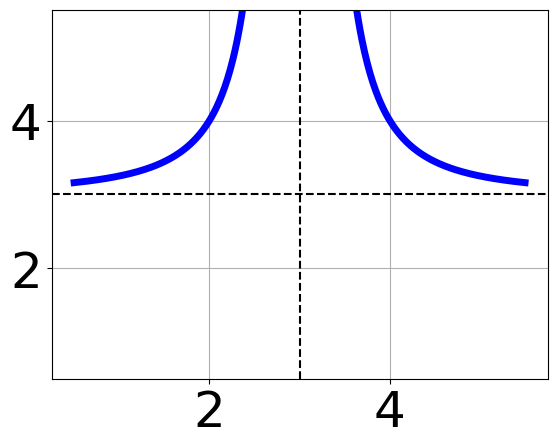
\includegraphics[width=0.3\textwidth]{../Figures/rationalEquationToGraphDC.png}
    \end{center}\begin{enumerate}[label=\Alph*.]
\begin{multicols}{2}
\item 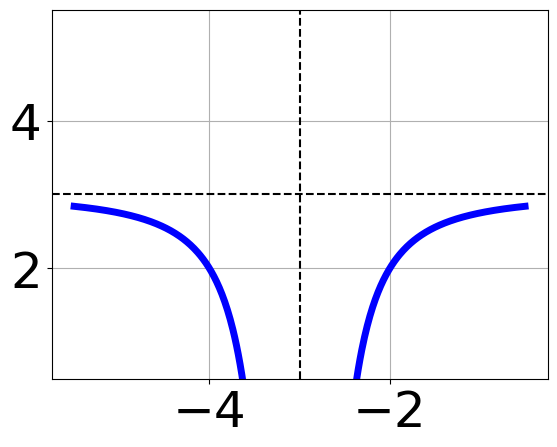
\includegraphics[width = 0.3\textwidth]{../Figures/rationalEquationToGraphAC.png}
\item 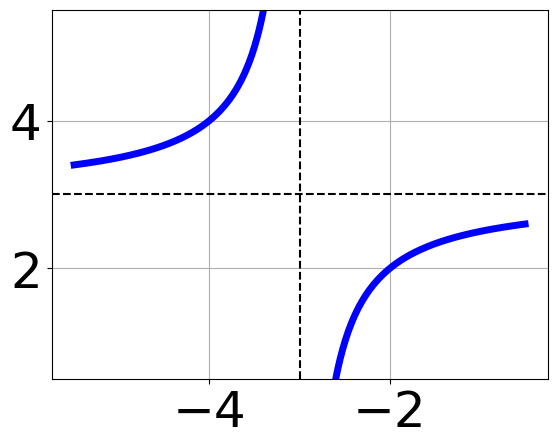
\includegraphics[width = 0.3\textwidth]{../Figures/rationalEquationToGraphBC.png}
\item 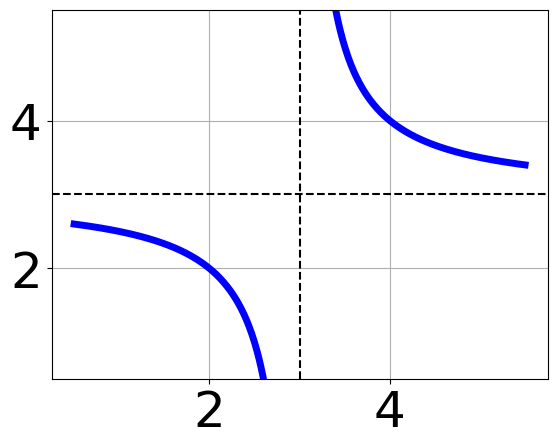
\includegraphics[width = 0.3\textwidth]{../Figures/rationalEquationToGraphCC.png}
\item 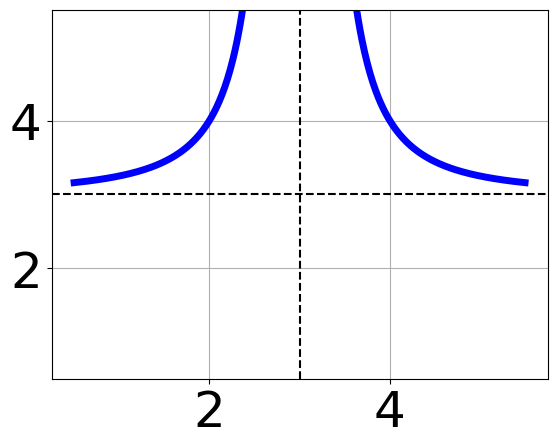
\includegraphics[width = 0.3\textwidth]{../Figures/rationalEquationToGraphDC.png}
\end{multicols}\item None of the above.\end{enumerate}
\textbf{General Comment:} Remember that the general form of a basic rational equation is $ f(x) = \frac{a}{(x-h)^n} + k$, where $a$ is the leading coefficient (and in this case, we assume is either $1$ or $-1$), $n$ is the degree (in this case, either $1$ or $2$), and $(h, k)$ is the intersection of the asymptotes.
}
\litem{
Choose the graph of the equation below.
\[ f(x) = \frac{1}{x + 2} - 2 \]The solution is the graph below, which is option D.
    \begin{center}
        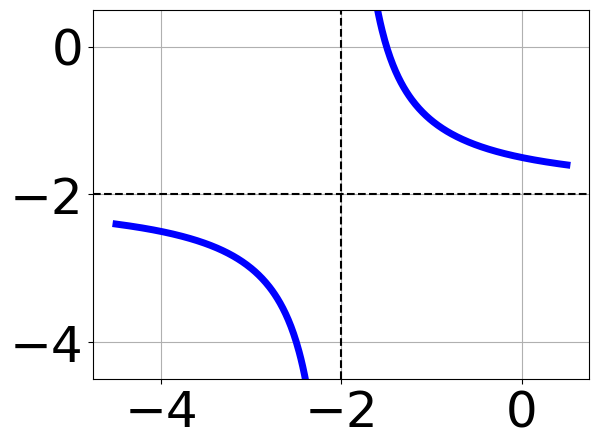
\includegraphics[width=0.3\textwidth]{../Figures/rationalEquationToGraphCopyDC.png}
    \end{center}\begin{enumerate}[label=\Alph*.]
\begin{multicols}{2}
\item 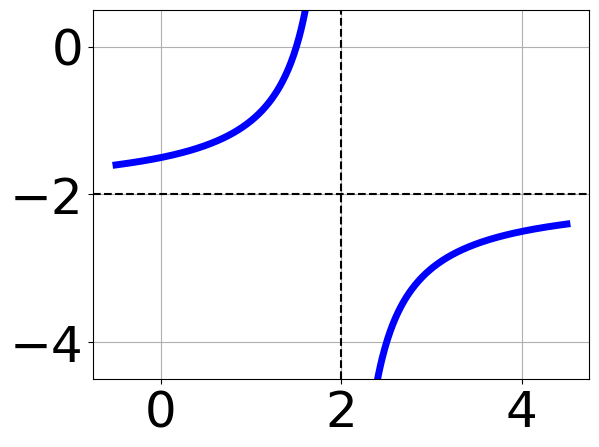
\includegraphics[width = 0.3\textwidth]{../Figures/rationalEquationToGraphCopyAC.png}
\item 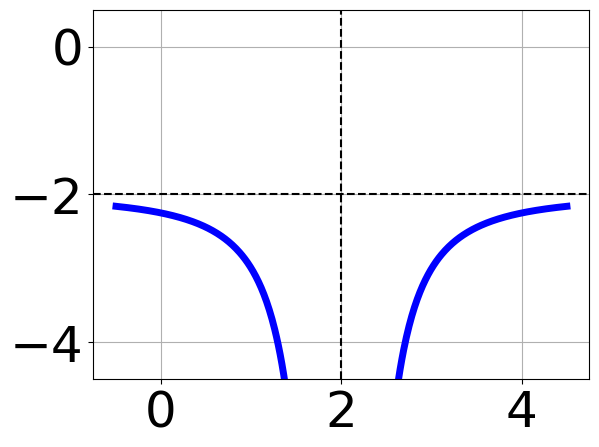
\includegraphics[width = 0.3\textwidth]{../Figures/rationalEquationToGraphCopyBC.png}
\item 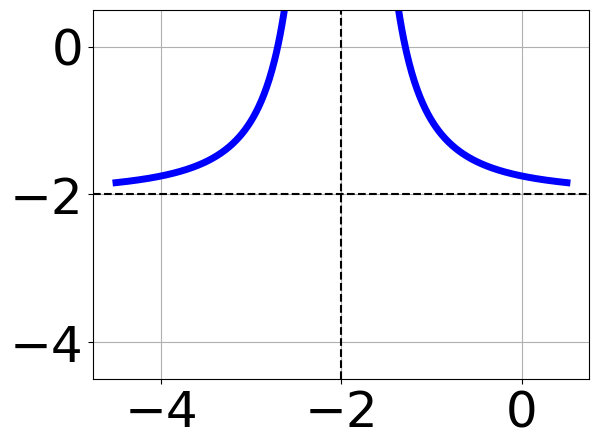
\includegraphics[width = 0.3\textwidth]{../Figures/rationalEquationToGraphCopyCC.png}
\item 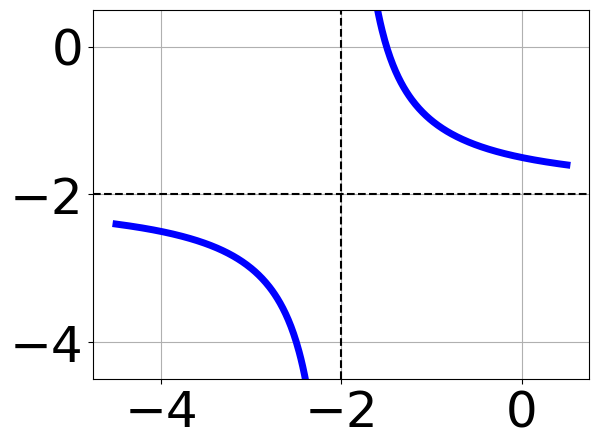
\includegraphics[width = 0.3\textwidth]{../Figures/rationalEquationToGraphCopyDC.png}
\end{multicols}\item None of the above.\end{enumerate}
\textbf{General Comment:} Remember that the general form of a basic rational equation is $ f(x) = \frac{a}{(x-h)^n} + k$, where $a$ is the leading coefficient (and in this case, we assume is either $1$ or $-1$), $n$ is the degree (in this case, either $1$ or $2$), and $(h, k)$ is the intersection of the asymptotes.
}
\litem{
Choose the equation of the function graphed below.

\begin{center}
    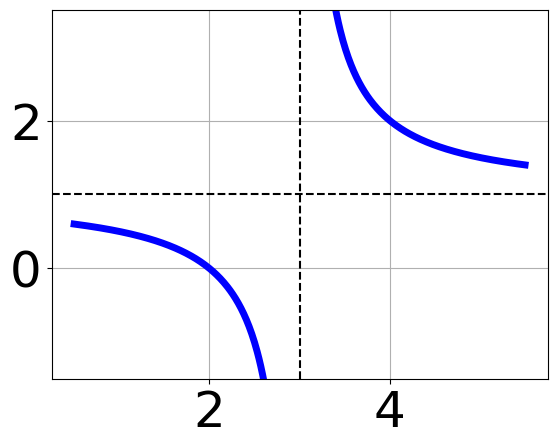
\includegraphics[width=0.5\textwidth]{../Figures/rationalGraphToEquationC.png}
\end{center}


The solution is \( f(x) = \frac{1}{x - 3} + 1 \), which is option C.\begin{enumerate}[label=\Alph*.]
\item \( f(x) = \frac{-1}{x + 3} + 1 \)

Corresponds to using the general form $f(x) = \frac{a}{x+h}+k$ and the opposite leading coefficient.
\item \( f(x) = \frac{-1}{(x + 3)^2} + 1 \)

Corresponds to thinking the graph was a shifted version of $\frac{1}{x^2}$, using the general form $f(x) = \frac{a}{x+h}+k$, and the opposite leading coefficient.
\item \( f(x) = \frac{1}{x - 3} + 1 \)

This is the correct option.
\item \( f(x) = \frac{1}{(x - 3)^2} + 1 \)

Corresponds to thinking the graph was a shifted version of $\frac{1}{x^2}$.
\item \( \text{None of the above} \)

This corresponds to believing the vertex of the graph was not correct.
\end{enumerate}

\textbf{General Comment:} Remember that the general form of a basic rational equation is $ f(x) = \frac{a}{(x-h)^n} + k$, where $a$ is the leading coefficient (and in this case, we assume is either $1$ or $-1$), $n$ is the degree (in this case, either $1$ or $2$), and $(h, k)$ is the intersection of the asymptotes.
}
\litem{
Choose the equation of the function graphed below.

\begin{center}
    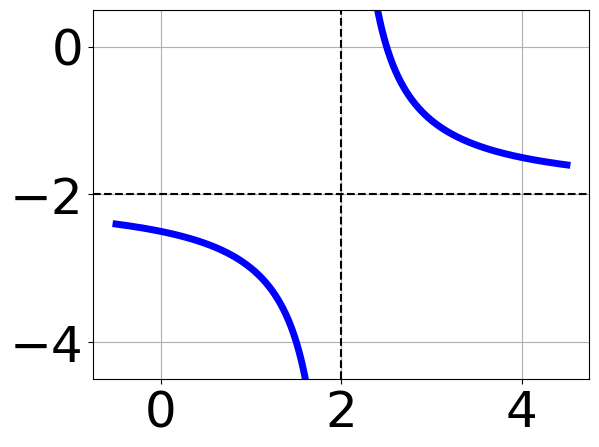
\includegraphics[width=0.5\textwidth]{../Figures/rationalGraphToEquationCopyC.png}
\end{center}


The solution is \( \text{None of the above as it should be } f(x) = \frac{1}{x - 2} - 2 \), which is option E.\begin{enumerate}[label=\Alph*.]
\item \( f(x) = \frac{1}{x + 2} - 5 \)

The $x$- and $y$-value of the equation does not match the graph.
\item \( f(x) = \frac{-1}{x - 2} - 5 \)

Corresponds to using the general form $f(x) = \frac{a}{x-h}+k$, the opposite leading coefficient AND not noticing the $y$-value was wrong.
\item \( f(x) = \frac{1}{(x + 2)^2} - 5 \)

Corresponds to thinking the graph was a shifted version of $\frac{1}{x^2}$ not noticing the $y$-value was wrong.
\item \( f(x) = \frac{-1}{(x - 2)^2} - 5 \)

Corresponds to thinking the graph was a shifted version of $\frac{1}{x^2}$, using the general form $f(x) = \frac{a}{x-h}+k$, the opposite leading coefficient, AND not noticing the $y$-value was wrong.
\item \( \text{None of the above} \)

None of the equation options were the correct equation.
\end{enumerate}

\textbf{General Comment:} Remember that the general form of a basic rational equation is $ f(x) = \frac{a}{(x-h)^n} + k$, where $a$ is the leading coefficient (and in this case, we assume is either $1$ or $-1$), $n$ is the degree (in this case, either $1$ or $2$), and $(h, k)$ is the intersection of the asymptotes.
}
\litem{
Solve the rational equation below. Then, choose the interval(s) that the solution(s) belongs to.
\[ \frac{-10}{40x + 20} + 1 = \frac{-10}{40x + 20} \]The solution is \( \text{all solutions are invalid or lead to complex values in the equation.} \), which is option E.\begin{enumerate}[label=\Alph*.]
\item \( x \in [0,1.4] \)

$x = 0.500$, which corresponds to not distributing the factor $40x + 20$ correctly when trying to eliminate the fraction.
\item \( x_1 \in [-0.9, -0.3] \text{ and } x_2 \in [-1.8,0.3] \)

$x = -0.500 \text{ and } x = -0.500$, which corresponds to getting the correct solution and believing there should be a second solution to the equation.
\item \( x_1 \in [-0.9, -0.3] \text{ and } x_2 \in [-0.4,1.5] \)

$x = -0.500 \text{ and } x = 0.500$, which corresponds to getting the correct solution and believing there should be a second solution to the equation.
\item \( x \in [-0.5,1.5] \)

$x = -0.500$, which corresponds to not checking if this value leads to dividing by 0 in the original equation and thus is not a valid solution.
\item \( \text{All solutions lead to invalid or complex values in the equation.} \)

*$x = -0.500$ leads to dividing by 0 in the original equation and thus is not a valid solution, which is the correct option.
\end{enumerate}

\textbf{General Comment:} Distractors are different based on the number of solutions. Remember that after solving, we need to make sure our solution does not make the original equation divide by zero!
}
\litem{
Solve the rational equation below. Then, choose the interval(s) that the solution(s) belongs to.
\[ \frac{6}{-2x -9} + -3 = \frac{-4}{18x + 81} \]The solution is \( x = -5.426 \), which is option B.\begin{enumerate}[label=\Alph*.]
\item \( x \in [3.1,3.8] \)

$x = 3.574$, which corresponds to not distributing the factor $-2x -9$ correctly when trying to eliminate the fraction.
\item \( x \in [-5.43,-4.43] \)

* $x = -5.426$, which is the correct option.
\item \( \text{All solutions lead to invalid or complex values in the equation.} \)

This corresponds to thinking $x = -5.426$ leads to dividing by zero in the original equation, which it does not.
\item \( x_1 \in [-6.7, -5.6] \text{ and } x_2 \in [-5.43,-3.43] \)

$x = -6.167 \text{ and } x = -5.426$, which corresponds to getting the correct solution and believing there should be a second solution to the equation.
\item \( x_1 \in [-5.5, -5.2] \text{ and } x_2 \in [2.57,4.57] \)

$x = -5.426 \text{ and } x = 3.574$, which corresponds to getting the correct solution and believing there should be a second solution to the equation.
\end{enumerate}

\textbf{General Comment:} Distractors are different based on the number of solutions. Remember that after solving, we need to make sure our solution does not make the original equation divide by zero!
}
\litem{
Determine the domain of the function below.
\[ f(x) = \frac{6}{24x^{2} -38 x + 15} \]The solution is \( \text{All Real numbers except } x = 0.750 \text{ and } x = 0.833. \), which is option C.\begin{enumerate}[label=\Alph*.]
\item \( \text{All Real numbers except } x = a, \text{ where } a \in [0.71, 0.77] \)

All Real numbers except $x = 0.750$, which corresponds to removing only 1 value from the denominator.
\item \( \text{All Real numbers.} \)

This corresponds to thinking the denominator has complex roots or that rational functions have a domain of all Real numbers.
\item \( \text{All Real numbers except } x = a \text{ and } x = b, \text{ where } a \in [0.71, 0.77] \text{ and } b \in [0.82, 0.85] \)

All Real numbers except $x = 0.750$ and $x = 0.833$, which is the correct option.
\item \( \text{All Real numbers except } x = a, \text{ where } a \in [11.91, 12.1] \)

All Real numbers except $x = 12.000$, which corresponds to removing a distractor value from the denominator.
\item \( \text{All Real numbers except } x = a \text{ and } x = b, \text{ where } a \in [11.91, 12.1] \text{ and } b \in [29.9, 30.18] \)

All Real numbers except $x = 12.000$ and $x = 30.000$, which corresponds to not factoring the denominator correctly.
\end{enumerate}

\textbf{General Comment:} Recall that dividing by zero is not a real number. Therefore the domain is all real numbers \textbf{except} those that make the denominator 0.
}
\litem{
Solve the rational equation below. Then, choose the interval(s) that the solution(s) belongs to.
\[ \frac{-2x}{2x + 2} + \frac{-4x^{2}}{-12x^{2} -18 x -6} = \frac{-7}{-6x -3} \]The solution is \( \text{All solutions are invalid or lead to complex values in the equation.} \), which is option C.\begin{enumerate}[label=\Alph*.]
\item \( x_1 \in [-1.47, -1.27] \text{ and } x_2 \in [-0.26,0.74] \)

$x = -1.321 \text{ and } x = 0.071$, which corresponds to making the discriminant from the Quadratic Formula positive to avoid complex solutions.
\item \( x \in [-0.58,-0.31] \)

$x = -0.500$, which corresponds to solving $-6x -3 = 0$ and treating it as a solution to the equation.
\item \( \text{All solutions lead to invalid or complex values in the equation.} \)

* The equation leads to solving $16x^{2} +20 x + 14=0$, which leads to complex solutions. This is the correct option.
\item \( x_1 \in [-1.18, -0.67] \text{ and } x_2 \in [-1.64,-0.49] \)

$x = -1.000 \text{ and } x = -0.500$, which corresponds to solving $2x + 2 = 0$ and $-6x -3 = 0$ and treating them as solutions to the equation.
\item \( x \in [-1.18,-0.67] \)

$x = -1.000$, which corresponds to solving $2x + 2 = 0$ and treating it as a solution to the equation.
\end{enumerate}

\textbf{General Comment:} Distractors are different based on the number of solutions. Remember that after solving, we need to make sure our solution does not make the original equation divide by zero!
}
\litem{
Solve the rational equation below. Then, choose the interval(s) that the solution(s) belongs to.
\[ \frac{-3x}{-6x + 5} + \frac{-2x^{2}}{-12x^{2} +52 x -35} = \frac{-4}{2x -7} \]The solution is \( \text{There are two solutions: } x = 1.405 \text{ and } x = -1.780 \), which is option D.\begin{enumerate}[label=\Alph*.]
\item \( x \in [3.15,4.34] \)


\item \( x \in [-3.35,-0.26] \)


\item \( x_1 \in [0.39, 3.08] \text{ and } x_2 \in [-1.17,7.83] \)


\item \( x_1 \in [0.39, 3.08] \text{ and } x_2 \in [-2.78,-0.78] \)

* $x = 1.405 \text{ and } x = -1.780$, which is the correct option.
\item \( \text{All solutions lead to invalid or complex values in the equation.} \)


\end{enumerate}

\textbf{General Comment:} Distractors are different based on the number of solutions. Remember that after solving, we need to make sure our solution does not make the original equation divide by zero!
}
\end{enumerate}

\end{document}